\documentclass{home_assignment}
\usepackage[inline]{enumitem}
\usepackage{amsthm}
\usepackage{tikz}
\usepackage{pgfplots}
\pgfplotsset{compat=1.17}
\tikzset{
    black node/.style={draw, circle, fill=black, inner sep=0pt,
    minimum width=2.5pt}
}
\pgfplotsset{every tick label/.append style={font=\small}}
\newcommand{\fourierplotten}{
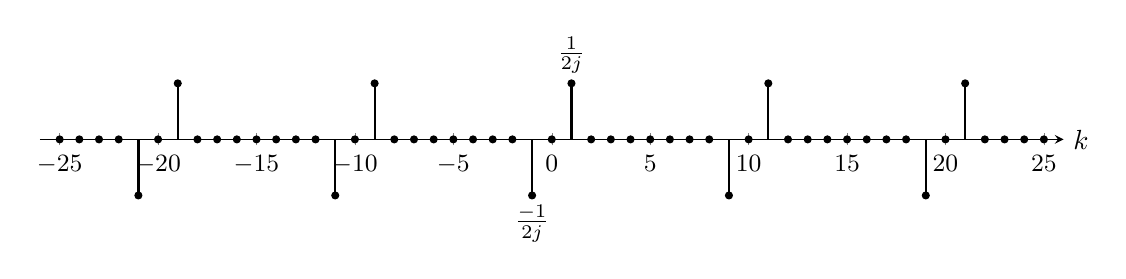
\begin{tikzpicture}
  \begin{axis}[
      axis x line=middle,
      axis y line=none,
      xmin=-26,xmax=26,
      ymin=-2,ymax=2,
      x=0.25cm,
      xlabel=$k$,
      xlabel style = {anchor=west},
    ];
     info{
    \node at (1,0.5) [anchor=south] {$\frac{1}{2j}$};
     \node at (-1,-0.5) [anchor=north] {$\frac{-1}{2j}$};
    };
    \foreach \x in{-19,-9,1,11,21}{
    \addplot[thick,black,mark=none,] coordinates {(\x,0) (\x,0.5)};
     \edef\temp{\noexpand\node at (\x,0.5) [black node]{}; } \temp
     }
     \foreach \x in{-21,-11,-1,9,19}{
    \addplot[thick,black,mark=none,] coordinates {(\x,0) (\x,-0.5)};
     \edef\temp{\noexpand\node at (\x,-0.5) [black node]{}; } \temp
     }
    \foreach \i in {-25,-24,-23,-22,-20,-18,-17,-16,-15,-14,-13,-12,-10,-8,-7,
    -6,-5,-4,-3,-2,0,2,3,4,5,6,7,8,10,12,13,14,15,16,17,18,20,22,23,24,25} { 
     \edef\temp{\noexpand\node at (\i,0) [black node]{}; } \temp
    }
  \end{axis}
\end{tikzpicture}
}
\newcommand{\fourierplotfifteen}{
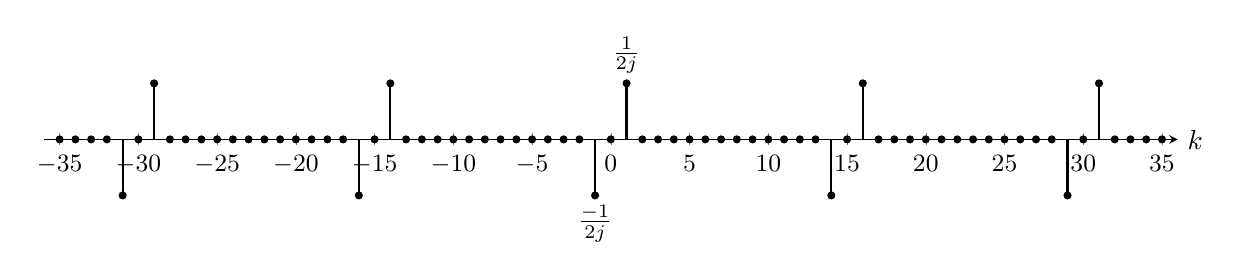
\begin{tikzpicture}
  \begin{axis}[
      axis x line=middle,
      axis y line=none,
      xmin=-36,xmax=36,
      ymin=-2,ymax=2,
      x=0.2cm,
      xlabel=$k$,
      xlabel style = {anchor=west},
    ]
     info{
    \node at (1,0.5) [anchor=south] {$\frac{1}{2j}$};
     \node at (-1,-0.5) [anchor=north] {$\frac{-1}{2j}$};
    };
    \foreach \x in{-29,-14,1,16,31}{
    \addplot[thick,black,mark=none,] coordinates {(\x,0) (\x,0.5)};
    \edef\temp{\noexpand\node at (\x,0.5) [black node]{}; } \temp
    }
     \foreach \x in{-31,-16,-1,14,29}{
    \addplot[thick,black,mark=none,] coordinates {(\x,0) (\x,-0.5)};
    \edef\temp{\noexpand\node at (\x,-0.5) [black node]{}; } \temp}
    \foreach \i in {-35,-34,-33,-32,-30,-28,-27,-26,-25,-24,-23,-22,-21,-20,-19,-18,-17,-15,-13,-12,-11,
    -10,-9,-8,-7,-6,-5,-4,-3,-2,0,2,3,4,5,6,7,8,9,10,11,12,13,15,17,18,19,20,21,22,23,24,25,26,27,28,30,32,33,34,35} { 
     \edef\temp{\noexpand\node at (\i,0) [black node]{}; } \temp
    }
  \end{axis}
\end{tikzpicture}
}
\newcommand{\squarewave}{
\begin{tikzpicture}
  \begin{axis}[
      axis x line=middle,
      axis y line=none,
      xmin=-13,xmax=13,
      ymin=-2,ymax=2,
      ticks=none,
      x=0.5cm,
      xlabel=$k$,
      xlabel style = {anchor=west},
    ];
  info{
    \node at (0,1) [anchor=south east] {$1$};
   
    };
    \foreach \x in{-8,-7,-6,-5,0,1,2,3,8,9,10,11}{
    \addplot[thick,black,mark=none,] coordinates {(\x,0) (\x,1)};
     \edef\temp{\noexpand\node at (\x,1) [black node]{}; } \temp
    }
    \foreach \i in {-12,-11,-10,-9,-4,-3,-2,-1,4,5,6,7,12} { 
     \edef\temp{\noexpand\node at (\i,0) [black node]{}; } \temp
    }
    \draw[decorate, decoration={brace,mirror, amplitude=5pt, raise=1pt}] (0,0) -- (3,0) node[midway,below=5pt,xshift=-1mm, ] {$N_p$};
     \draw[decorate, decoration={brace,mirror, amplitude=5pt, raise=18pt}] (-4,0) -- (3,0) node[midway,below=5pt,yshift=-19pt] {$N$};
  \end{axis}
\end{tikzpicture}
}

\newtheorem{theorem}{Property}
\newtheorem{subtheorem}{Symmetry Property}[theorem]
\begin{document}
\titlePage{Signal Analysis Asssignment \#5}{October 5, 2020}{Dr. Dibakar Raj Panta}
\problem{Show, if $x(t)$ is real and odd, then its Fourier series coefficients are purely imaginary and odd.}
\solution{The question suggests that the signal $x(t)$ is real and odd which means, $x(t)=-x(-t)$. We can write the Fourier series coefficients for the signal $x(t)$ as:
\begin{equation}
C_k=\frac{1}{T_0}\int_{-T_0/2}^{T_0/2}x(t) e^{-jk\omega_0 t}dt
\label{eqn:Ck}
\end{equation}
\textit{Method 1:}\\
  Rewriting Eq.(\ref{eqn:Ck}) using the Euler's identity as,
  \begin{equation*}
  \begin{aligned}
  C_k&=\frac{1}{T_0}\int_{-T_0/2}^{T_0/2}x(t)cos(k\omega_0 t)dt-j\frac{1}{T_0}\int_{-T_0/2}^{T_0/2}x(t)sin(k\omega_0 t)dt\\
  &=0-j\frac{1}{T_0}\int_{-T_0/2}^{T_0/2}x(t)sin(k\omega_0 t)dt\\
  &=-j\frac{1}{T_0}\int_{-T_0/2}^{T_0/2}x(t)sin(k\omega_0 t)dt
  \end{aligned}  
  \end{equation*}
Since $x(t)cos(k\omega_0 t)$ is odd the resulting integration is 0. From the above equation for $C_k$ \textbf{we can conclude that, the fourier series coefficients are odd since $C_k=-C_{-k}$ and purely imaginary.}\\\\
\textit{Method 2:}\\
Rewriting Eq.(\ref{eqn:Ck}) by separating the limits of integration as,
\begin{equation*}
  \begin{aligned}
  C_k&=\frac{1}{T_0}\int_{-T_0/2}^{0}x(t)e^{-jk\omega_0 t}dt+\frac{1}{T_0}\int_{0}^{T_0/2}x(t)e^{-jk\omega_0 t}dt\\
  &=\frac{1}{T_0}\int_{0}^{T_0/2}x(-t)e^{jk\omega_0 t}dt+\frac{1}{T_0}\int_{0}^{T_0/2}x(t)e^{-jk\omega_0 t}dt\\
   &=-\frac{1}{T_0}\int_{0}^{T_0/2}x(t)e^{jk\omega_0 t}dt+\frac{1}{T_0}\int_{0}^{T_0/2}x(t)e^{-jk\omega_0 t}dt\\
    &=\frac{1}{T_0}\int_{0}^{T_0/2}x(t)\left[e^{-jk\omega_0 t}-e^{jk\omega_0 t}\right]dt\\
    &=\frac{1}{T_0}\int_{0}^{T_0/2}x(t)[-2jsin(k\omega_0 t)]dt\\
     &=-2j\frac{1}{T_0}\int_{0}^{T_0/2}x(t)sin(k\omega_0 t)dt
  \end{aligned}  
  \end{equation*}
  From this equation for $C_k$ it is clear that \textbf{for a signal $x(t)$ that is real and odd, the fourier series coefficients are odd and purely imaginary.}
}
\problem{Plot the fourier series coefficients for the discrete time signal $x[n]=sin\left(\frac{2\pi}{N}\right)n$ for: 
\begin{enumerate*}[label=(\roman*)]
\item $N=10$    
\item $N=15$
\end{enumerate*}
}
\clearpage
\solution{
\begin{enumerate*}[label=(\roman*)]
\item $N=10$
\end{enumerate*}
\begin{figure}[H]
\centering
\fourierplotten
\caption{Plot for $a_k$ for $N=10$}
\label{fig:n=10}
\end{figure}
\begin{enumerate*}[label=(\roman*)]
\setcounter{enumi}{1}
\item $N=15$
\end{enumerate*}
\begin{figure}[H]
\centering
\fourierplotfifteen
\caption{Plot for $a_k$ for $N=15$}
\label{fig:n=15}
\end{figure}
}
\problem{Find the fourier series coefficients for the discrete-time periodic square wave.}
\solution{Considering a periodic square wave with arbitrary period $N$ and pulse width of $N_p$ samples for a more generic result.
\begin{figure}[H]
\centering
\squarewave
\caption{Plot for discrete time periodic square wave}
\label{fig:sqwave}
\end{figure}
The fourier series coefficients for any discrete time signal is given by,
\begin{equation}
C_k=\frac{1}{N}\sum_{n=0}^{N-1}x[n]e^{-jkn\frac{2\pi}{N}}
\label{eqn:sqwave}
\end{equation}
From Fig.(\ref{fig:sqwave}) it is clear that, the Eq.(\ref{eqn:sqwave}) is non-zero for period $N_p$ and 0 for any other period. So, we can rewrite Eq.(\ref{eqn:sqwave}) as,
\begin{equation*}
C_k=\frac{1}{N}\sum_{n=0}^{N_p-1}e^{-jkn\frac{2\pi}{N}}
\end{equation*}
For $k=0$, 
\begin{equation*}
\begin{aligned}
C_0&=\frac{1}{N}\sum_{n=0}^{N_p-1}e^0\\
&=\frac{N_p}{N}
\end{aligned}
\end{equation*}
which is the average value of the signal averaged over the period $N$.
For $k\neq 0$
\begin{equation*}
\begin{aligned}
C_k&=\frac{1}{N}\sum_{n=0}^{N_p-1}\left(e^{-jk\frac{2\pi}{N}}\right)^n\\
&=\frac{1}{N}\left[\frac{1-\left(e^{-jk\frac{2\pi}{N}}\right)^{N_p}}{1-\left(e^{-jk\frac{2\pi}{N}}\right)}\right]\\
&=\frac{1}{N}\left[\frac{e^{-jkN_p\frac{\pi}{N}}\left(e^{jkN_p\frac{\pi}{N}}-e^{-jkN_p\frac{\pi}{N}}\right)}{e^{-jk\frac{\pi}{N}}\left(e^{jk\frac{\pi}{N}}-e^{-jk\frac{\pi}{N}}\right)}\right]\\
&=\frac{1}{N}\left[\frac{e^{-jkN_p\frac{\pi}{N}}\left\lbrace 2jsin\left(kN_p\frac{\pi}{N}\right)\right\rbrace}{e^{-jk\frac{\pi}{N}}\left\lbrace 2jsin\left(k\frac{\pi}{N}\right)\right\rbrace}\right]\\
&=\frac{1}{N}\left[\frac{sin\left(k\frac{N_p \pi}{N}\right)}{sin\left(k \frac{\pi}{N}\right)}\right]e^{-jk(N_p -1)\frac{\pi}{N}}
\end{aligned}
\end{equation*}
Overall, we can write,
\begin{equation}
C_k=\begin{cases}
\frac{N_p}{N}, & k=0\\
\frac{1}{N}\left[\frac{sin\left(k\frac{N_p \pi}{N}\right)}{sin\left(k \frac{\pi}{N}\right)}\right]e^{-jk(N_p -1)\frac{\pi}{N}}, & k \neq 0
\end{cases}
\end{equation}
This result suggests that the fourier series coefficient of a periodic square wave signal is a digital sinc signal.
}
\problem{State and prove DTFS properties.}
\solution{
If $\fourier{x[n]}$ denotes the fourier series transformation of $x[n]$ into its fourier coefficients such that,
\begin{equation}
\fourier{x[n]}=c_{k},\quad \text{where}\quad c_{k}=\frac{1}{N} \sum_{n=0}^{N-1} x[n] e^{-\left(j \frac{2 \pi}{N} k n\right)}
\label{eqn:DTFS}
\end{equation}
\begin{theorem}[Linearity]
If $\fourier{x[n]}=a_k$ and $\fourier{y[n]}=b_k$, then
\begin{equation*}
\fourier{Ax[n]+By[n]}=Aa_k+Bb_k
\end{equation*}
\end{theorem}
\begin{proof}
This can be proved based on the properties of a summation over a limit.
\begin{equation*}
\begin{aligned} 
\fourier{Ax[n]+By[n]} &=\sum_{n=0}^{N-1}(Ax[n]+By[n]) e^{-\left(j \omega_{0} k n\right)} \\ 
&=\frac{1}{N} A\sum_{n=0}^{N-1} x[n] e^{-\left(j \omega_{0} k n\right)}+\frac{1}{N} B\sum_{n=0}^{N-1} y[n] e^{-\left(j \omega_{0} k n\right)} \\ 
&=Aa_{k}+Bb_{k}\\ 
\end{aligned}
\end{equation*}
\end{proof}
\begin{theorem}[Time Shifting]
Shifting a signal $x[n]$ by $n_0$ results in a phase shift of fourier coefficients such that,
\begin{equation*}
\fourier{x[n-n_0]}=c_k e^{-(j\omega_0 k n_0)} 
\end{equation*}
\end{theorem}
\begin{proof}
\begin{equation*}
\begin{aligned} 
\fourier{\left(x\left[n-n_{0}\right]\right)} &=\frac{1}{N} \sum_{n=0}^{N-1} x\left[n-n_{0}\right] e^{-\left(j \omega_{0} k n\right)}\\ 
&=\frac{1}{N} \sum_{n-n_0=0}^{N-n_{0}-1} x\left[n-n_{0}\right] e^{-\left(j \omega_{0} k\left(n-n_{0}\right)\right)} e^{-\left(j \omega_{0} k n_{0}\right)} \\ 
&=\frac{1}{N} \sum_{n-n_{0}=0}^{N-n_{0}-1} x[\tilde{n}] e^{-\left(j \omega_{0} k \tilde{n}\right)} e^{-\left(j \omega_{0} k n_{0}\right)} \quad, where \quad \tilde{n}=n-n_0 \\ 
&=c_{k}e^{-\left(j \omega_{0} k n_0\right)}
\end{aligned}
\end{equation*}
If $c_{k}=\left|c_{k}\right| e^{j \angle\left(c_{k}\right)}$ then, the magnitude is given by, 
\begin{equation}
\left|c_ke^{-\left(j \omega_{0} k n_{0}\right)}\right|=\left|c_{k}\right|\left|e^{-\left(j \omega_{0} k n_{0}\right)}\right|=\left|c_{k}\right|
\label{eqn:shiftmag}
\end{equation}
Likewise, the phase is given by, 
\begin{equation}
\angle\left(c_ke^{-\left(j \omega_{0} n_{0} k\right)}\right)=\angle\left(c_{k}\right)-\omega_{0} n_{0} k 
\label{eqn:shiftphase}
\end{equation}
Eq.(\ref{eqn:shiftphase}) clearly shows that the shift of $n_0$ in the signal $x[n]$ results in a phase shift for the fourier coefficients.
\end{proof}
\begin{theorem}[Frequency Shifting]
The frequency shift of a signal $x[n]$ results in an equivalent shift in its fourier coefficient spectrum such that,
\begin{equation*}
\fourier{x[n]e^{jm\frac{2\pi}{N}n}}=c_{k-m}
\end{equation*}
\end{theorem}
\begin{proof}
From Eq.(\ref{eqn:DTFS}) we can write,
\begin{equation*}
\begin{aligned}
\fourier{x[n]e^{jm\frac{2\pi}{N}n}}&=\frac{1}{N}\sum_{n=0}^{N-1}x[n]e^{jm\frac{2\pi}{N}n}e^{-jk\frac{2\pi}{N}n}\\
&=\frac{1}{N}\sum_{n=0}^{N-1}x[n]e^{-j\frac{2\pi}{N}n(k-m)}\\
&=c_{k-m}
\end{aligned}
\end{equation*}
\end{proof}
\begin{theorem}[Conjugation]
The fourier coefficient for a conjugate of a signal $x[n]$ is also an equivalent conjugate such that,
$$
\fourier{x^*[n]}=c^*_{-k}
$$
\end{theorem}
\begin{proof}
To prove this, we start from the Eq.(\ref{eqn:DTFS})
$$
\begin{aligned}
c_k&=\frac{1}{N}\sum_{n=0}^{N-1}x[n]e^{-jk\frac{2\pi}{N}n}\\
\Rightarrow \quad c^*_k&=\frac{1}{N}\sum_{n=0}^{N-1}x^*[n]e^{jk\frac{2\pi}{N}n}\\
\Rightarrow \quad c^*_{-k}&=\frac{1}{N}\sum_{n=0}^{N-1}x^*[n]e^{-jk\frac{2\pi}{N}n}\\
\Rightarrow \quad c^*_{-k}&=\fourier{x^*[n]}
\end{aligned}
$$
\end{proof}
\begin{theorem}[Time Reversal]
The time reversal of a signal $x[n]$ results in an equivalent reversal in its fourier coefficient spectrum such that,
$$
\fourier{x[-n]}=c_{-k}
$$
\end{theorem}
\begin{proof}
To prove this, we start off as,
$$
\begin{aligned}
\fourier{x[-n]}&=\frac{1}{N}\sum_{n=0}^{N-1}x[-n]e^{-jk\frac{2\pi}{N}n}\\
&=\frac{1}{N}\sum_{\tilde{n}=0}^{N-1}x[\tilde{n}]e^{jk\frac{2\pi}{N}\tilde{n}}\quad where,\quad \tilde{n}=-n,\\
&=\frac{1}{N}\sum_{\tilde{n}=0}^{N-1}x[\tilde{n}]e^{-j(-k)\frac{2\pi}{N}\tilde{n}}\\
&=c_{-k}
\end{aligned}
$$
\end{proof}
\begin{theorem}[Multiplication]
Signal multiplication in time domain results in a DT circular convolution in the frequency domain. If $x[n]$ and $y[n]$ are two signals with fourier coefficients $a_k$ and $b_k$ respectively, the signal multiplication $z[n]=x[n]y[n]$ has the fourier series coefficients $c_k$ such that,
$$c_k=\sum_{l=0}^{N-1} a_{l} b_{k-l}
$$
\end{theorem}
\begin{proof}
$$\begin{aligned}
c_{k} &=\frac{1}{N} \sum_{n=0}^{N-1} x[n] y[n] e^{-\left(j \omega_{0} k n\right)} \\ 
&=\frac{1}{N} \sum_{n=0}^{N-1} \sum_{l=0}^{N-1} a_{l} e^{j \omega_{0} l n} y[n] e^{-\left(j \omega_{0} k n\right)}\\ 
&=\sum_{l=0}^{N-1} a_{l}\left(\frac{1}{N} \sum_{n=0}^{N-1} y[n] e^{-\left(j \omega_{0}(k-l) n\right)}\right) \\ 
&=\sum_{l=0}^{N-1} a_{l} b_{k-l} 
\end{aligned} $$
\enlargethispage{\baselineskip}
\end{proof}
\begin{theorem}[Periodic Convolution]
The periodic convolution of signals in the time domain results in the multiplication of their fourier coefficients. If If $x[n]$ and $y[n]$ are two signals with fourier coefficients $a_k$ and $b_k$ respectively, then the periodic convolution $\sum_{m=0}^{N-1}x[m]y[n-m]$ has the fourier coefficient $c_k$ such that
$$
c_k=Na_kb_k
$$
\end{theorem}
\begin{proof}
To prove this, we start off as,
$$
\begin{aligned}
c_k=&\fourier{\sum_{m=0}^{N-1}x[m]y[n-m]}\\
&=\frac{1}{N}\sum_{n=0}^{N-1} \sum_{m=0}^{N-1} x[m]y[n-m] e^{-\left(j \frac{2 \pi}{N} k n\right)}\\
&=N\left[\left\lbrace \frac{1}{N}\sum_{m=0}^{N-1} x[m]e^{-\left(j \frac{2 \pi}{N} k m\right)}\right\rbrace\left\lbrace\frac{1}{N}\sum_{n-m=0}^{N-m-1}y[n-m] e^{-\left(j \frac{2 \pi}{N} k (n-m)\right)}\right\rbrace\right]\\
&=Na_kb_k
\end{aligned}
$$
\end{proof}
\begin{theorem}[First Difference]
For a discrete time signal $x[n]$,
$$\fourier{x[n]-x[n-1]}=c_k\left(1-e^{-jk\frac{2\pi}{N}}\right)$$
\end{theorem}
\begin{proof}
To prove the first difference property, Linearity and Time Shifting properties are essential.
$$
\begin{aligned}
\fourier{x[n]-x[n-1]}&=\frac{1}{N}\sum_{n=0}^{N-1}\left(x[n]-x[n-1]\right)e^{-jk\frac{2\pi}{N}n}\\
&=\frac{1}{N}\sum_{n=0}^{N-1}x[n]e^{-jk\frac{2\pi}{N}n}-\frac{1}{N}\sum_{n=0}^{N-1}x[n-1]e^{-jk\frac{2\pi}{N}n}\\
&=c_k-\frac{1}{N}\sum_{n-1=0}^{N-1}x[n-1]e^{-jk\frac{2\pi}{N}(n-1)}e^{-jk\frac{2\pi}{N}}\\
&=c_k-e^{-jk\frac{2\pi}{N}}\frac{1}{N}\sum_{\tilde{n}=0}^{N-1}x[\tilde{n}]e^{-jk\frac{2\pi}{N}(\tilde{n})}\quad where, \tilde{n}=n-1\\
&=c_k-c_ke^{-jk\frac{2\pi}{N}}\\&=c_k\left(1-e^{-jk\frac{2\pi}{N}}\right)
\end{aligned}
$$
\end{proof}
\begin{theorem}[Duality]
The duality theorem states that, for a signal $x[n]$ such that $x[n]=\sum_{k=0}^{N-1}c_ke^{jk\frac{2\pi}{N}n}$, the signal shows dual property for role change of $n$ and $k$ as,
$$
\fourier{c_n}=\frac{1}{N}x[-k]
$$
\end{theorem}
\begin{proof}
$$
\begin{aligned}
\fourier{c_n}&=\frac{1}{N}\sum_{n=0}^{N-1} c_n e^{-\left(j \frac{2 \pi}{N} k n\right)}\\
&=\frac{1}{N}\sum_{n=0}^{N-1} c_n e^{\left(j \frac{2 \pi}{N} (-k) n\right)}\\
&=\frac{1}{N}x[-k]
\end{aligned}
$$
\enlargethispage{\baselineskip}
\end{proof}
\begin{theorem}[Symmetry Properties]
A signal $x[n]$ has various symmetry properties for odd, even and real valued conditions as,
\end{theorem}
\begin{subtheorem}[Conjugate symmetry for real signal]
For a signal $x[n]$ such that $x[n]=x^*[n]$, we have,
$$c_k=c^*_{-k}$$
\end{subtheorem}
\begin{proof}
$$
\begin{aligned}
c_k&=\fourier{x[n]}\\
\Rightarrow c_k&=\frac{1}{N} \sum_{n=0}^{N-1} x[n] e^{-\left(j \frac{2 \pi}{N} k n\right)}\\
\Rightarrow c^*_k&=\frac{1}{N} \sum_{n=0}^{N-1} x^*[n] e^{\left(j \frac{2 \pi}{N} k n\right)}\\
\Rightarrow c^*_{k}&=\frac{1}{N} \sum_{n=0}^{N-1} x[n] e^{-\left(j \frac{2 \pi}{N} (-k) n\right)}\\
\Rightarrow  c^*_{k}&=c_{-k}\\
\Rightarrow  c_{k}&=c^*_{-k}
\end{aligned}
$$
\end{proof}
\begin{subtheorem}[Real and even signal]
For a signal $x[n]$ such that $x[n]=x[-n]$, the coefficients are real and even.
\end{subtheorem}
\begin{proof}
$$
\begin{aligned}
c_k&=\frac{1}{N} \sum_{n=0}^{N} x[n] e^{-\left(j \frac{2 \pi}{N} k n\right)}\\
&=\frac{1}{N} \sum_{n=0}^{N/2} x[n] e^{-\left(j \frac{2 \pi}{N} k n\right)}+\frac{1}{N} \sum_{N/2}^{N} x[n] e^{-\left(j \frac{2 \pi}{N} k n\right)}\\
&=\frac{1}{N} \sum_{-n=0}^{N/2} x[-n] e^{\left(j \frac{2 \pi}{N} k n\right)}+\frac{1}{N} \sum_{N/2}^{N} x[n] e^{-\left(j \frac{2 \pi}{N} k n\right)}\\
&=\frac{1}{N} \sum_{n=0}^{N/2} x[n] e^{\left(j \frac{2 \pi}{N} k n\right)}+\frac{1}{N} \sum_{N/2}^{N} x[n] e^{-\left(j \frac{2 \pi}{N} k n\right)}\\
&=\frac{1}{N} \sum_{n=0}^{N} x[n]\left\lbrace e^{\left(j \frac{2 \pi}{N} k n\right)}+e^{-\left(j \frac{2 \pi}{N} k n\right)}\right\rbrace\\
&=\frac{2}{N} \sum_{n=0}^{N} x[n]\left\lbrace cos\left(k\frac{2\pi}{N}n\right)\right\rbrace\\
\end{aligned}
$$
The above equation is indeed a real and even signal since there's no imaginary term and cosine signal is an even signal.\\
\end{proof}
\begin{subtheorem}[Real and odd signal]
For a signal $x[n]$ such that $x[n]=-x[-n]$, the coefficients are purely imaginary and odd.
\end{subtheorem}
\begin{proof}
$$
\begin{aligned}
c_k&=\frac{1}{N} \sum_{n=0}^{N} x[n] e^{-\left(j \frac{2 \pi}{N} k n\right)}\\
&=\frac{1}{N} \sum_{n=0}^{N/2} x[n] e^{-\left(j \frac{2 \pi}{N} k n\right)}+\frac{1}{N} \sum_{N/2}^{N} x[n] e^{-\left(j \frac{2 \pi}{N} k n\right)}\\
&=\frac{1}{N} \sum_{-n=0}^{N/2} x[-n] e^{\left(j \frac{2 \pi}{N} k n\right)}+\frac{1}{N} \sum_{N/2}^{N} x[n] e^{-\left(j \frac{2 \pi}{N} k n\right)}\\
&=-\frac{1}{N} \sum_{n=0}^{N/2} x[n] e^{\left(j \frac{2 \pi}{N} k n\right)}+\frac{1}{N} \sum_{N/2}^{N} x[n] e^{-\left(j \frac{2 \pi}{N} k n\right)}\\
&=-\frac{1}{N} \sum_{n=0}^{N} x[n] \left\lbrace e^{\left(j \frac{2 \pi}{N} k n\right)}-e^{-\left(j \frac{2 \pi}{N} k n\right)}\right\rbrace\\
&=-\frac{2j}{N} \sum_{n=0}^{N} x[n]\left\lbrace sin\left(k\frac{2\pi}{N}n\right)\right\rbrace\\
\end{aligned}
$$
The above equation for $c_k$ is purely imaginary and is indeed an odd signal due to the sine function.
\end{proof}
}
\problem{Prove the parseval's relation for discrete time periodic signal.}
\solution{Parseval's relation for a discrete time periodic signal states that the average power in a periodic signal, say, $x[n]$ is equal to the sum of the average powers in all of its harmonic components.
\\Mathematically,
\begin{equation}
\frac{1}{N}\sum_{n=0}^{N-1}|x[n]|^2=\sum_{k=0}^{N-1}|c_k|^2
\label{eqn:parseval}
\end{equation}
\begin{proof}
To prove the Eq.(\ref{eqn:parseval}) we'll use the relation for $c_k$ from Eq.(\ref{eqn:DTFS})
$$
\begin{aligned}
\sum_{k=0}^{N-1}|c_k|^2&=\sum_{k=0}^{N-1}c_k c^*_k\\
&=\frac{1}{N} \sum_{k=0}^{N-1}c_k \sum_{n=0}^{N-1} x^*[n] e^{\left(j \frac{2 \pi}{N} k n\right)}\\
&=\frac{1}{N}\sum_{n=0}^{N-1} x^*[n] \left\lbrace\sum_{k=0}^{N-1} c_k e^{\left(j \frac{2 \pi}{N} k n\right)}\right\rbrace\\
&=\frac{1}{N}\sum_{n=0}^{N-1} x^*[n] x[n]\\&=\frac{1}{N}\sum_{n=0}^{N-1} |x[n]|^2
\end{aligned}
$$
\end{proof}
}
\end{document}